PIMS statistics is another feature for admin user only. For the statistics use case we tested for four different cases. All passed unit test and succeeded..
\\* 
%new line
The add user case passed unit testing successfully as seen in the figure bellow
\\* 
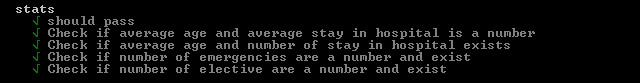
\includegraphics[width=350px]{./TestingDoc/Graphics/statsResults}
		
\subsubsection*{Conditions}
The following conditions had to be met for the statistics tests to pass.
	
\subsubsection*{Pre conditions}	
\begin{itemize}
		\item User must be logged in as admin.
		\item Object type has to be a digit.
\end{itemize}	

\subsubsection*{Post conditions}	
\begin{itemize}
		\item Statistical results are returned.
\end{itemize}	

Unit test code to validate the number of elective procedures is indeed a number.	

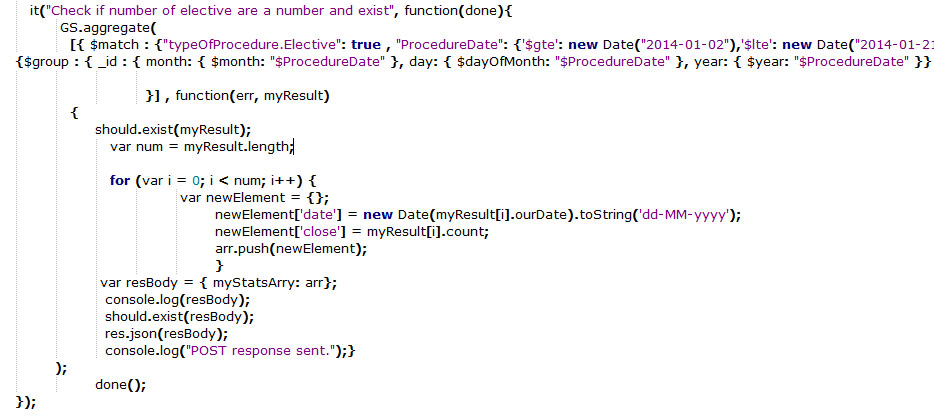
\includegraphics[width=350px]{./TestingDoc/Graphics/StatsChecknumexists}

Unit test codes to validate the average age and stay in hospitals are indeed numbers.	

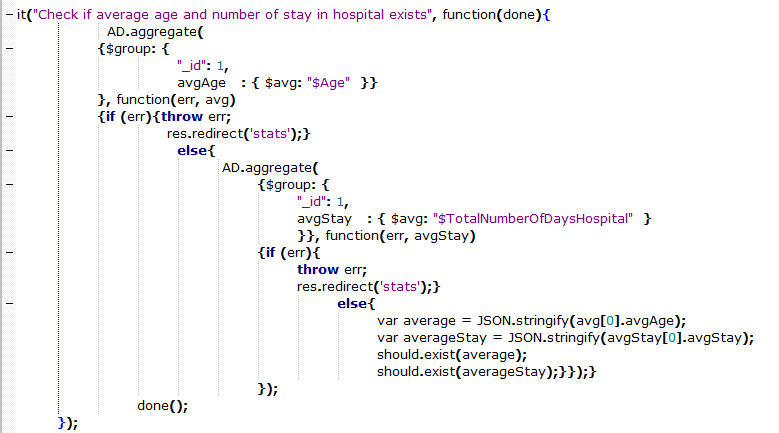
\includegraphics[width=350px]{./TestingDoc/Graphics/averageNumberStats}

\subsubsection*{Remark}
Statistics is the heaviest module the PIMS. More unit testing will be done to ensure accuracy, reliability and currency. For now all tests succeeded and passed.